\section{PAC-Bayesian Linear Regression}

In this section, we review Bayesian linear regression in the context of the
PAC-Bayes theory we have developed so far.

\subsection{Bayesian Inference Setup}

Suppose we are given data in the form of input-output pairs: $S = \{(x_1, y_1),
\ldots, (x_n, y_n)\}$ with $x_i \in [-1, 1]$ and $y_i \in \RR$ for $1 \leq i
\leq n$. Our goal is to find a function $f$ that fits this data, i.e.\ $y_i
\approx f(x_i)$.

\subsubsection{Likelihood Model}

We consider the following data model
\begin{equation}
  y = h_{\Vec{\theta}}(x) + \eta, \quad h_{\Vec{\theta}}(x) = \sum_{i = 1}^m
  \theta_i \phi_i(x), \quad \eta \sim \NormalDist(0, \sigma_\eta^2)
\end{equation}
$\Vec{\theta} = (\theta_1, \ldots, \theta_m)$ are the model parameters and
$\{\phi_i : 1 \leq i \leq m\}$ is a set of some of the basis functions for
$L^2[-1, 1]$, e.g.
\begin{itemize}
  \item
    Monomials, $\phi_i(x) = x^{i - 1}$
  \item
    Legendre polynomials, $\phi_i(x) = P_{i - 1}(x)$ normalized with $P_{i -
    1}(1) = 1$
\end{itemize}
For simplicity, let us assume $\sigma_\eta$ is constant. Let us denote
\begin{equation}
  \Vec{\phi}(x) = (\phi_1(x), \ldots, \phi_m(x)), \quad \Vec{x} = (x_1, \ldots,
  x_n), \quad \Vec{y} = (y_1, \ldots, y_n)
\end{equation}
Then we can write our likelihood model as
\begin{equation}
  x, y \mid \Vec{\theta} \sim \CD_X(x) \NormalDist(\Vec{\phi}(x)^\top
  \Vec{\theta}, \sigma_\eta^2) \implies -\log p(x, y) = \frac{1}{2
  \sigma_\eta^2} (y - \Vec{\phi}(x)^\top \Vec{\theta})^2 + \text{const.}
\end{equation}
Here $\CD_X(x)$ denotes the distribution of $x$; for the purpose of Bayesian
inference, we can ignore it completely. It will, however, be important in the
PAC-Bayes analysis.

Now, assuming the observations are i.i.d., we can write
\begin{equation}
  p(\Vec{x}, \Vec{y} \mid \Vec{\theta}) = \prod_{i = 1}^m \CD_X(x_i) p(y_i \mid
  \Vec{\phi}(x_i)^\top \Vec{\theta}, \sigma_\eta^2) \implies -\log p(\Vec{x},
  \Vec{y} \mid \Vec{\theta}) = \frac{1}{2 \sigma_\eta^2} \Norm{\Vec{y} -
  \Mat{\Phi}(\Vec{x})^\top \Vec{\theta}}^2 + \text{const.}
\end{equation}
where
\begin{equation}
  \Mat{\Phi}(\Vec{x}) =
  \begin{bmatrix}
    \Vec{\phi}(x_1) & \cdots & \Vec{\phi}(x_n)
  \end{bmatrix}
  =
  \begin{bmatrix}
    \phi_1(x_1) & \cdots & \phi_1(x_n) \\
    \vdots & \ddots & \vdots \\
    \phi_m(x_1) & \cdots & \phi_m(x_n)
  \end{bmatrix}
  \in \RR^{m \times n}
\end{equation}

\subsubsection{Prior Model}

We consider Gaussian priors on $\Vec{\theta}$:
\begin{equation}
  \Vec{\theta} \sim \NormalDist(\Vec{\mu}_0, \Mat{\Sigma}_0) \implies -\log
  p(\Vec{\theta}) = \frac{1}{2} (\Vec{\theta} - \Vec{\mu}_0)^\top
  \Mat{\Sigma}_0^{-1} (\Vec{\theta} - \Vec{\mu}_0) + \text{const.}
\end{equation}

\begin{figure}
  \begin{subfigure}{\textwidth}
    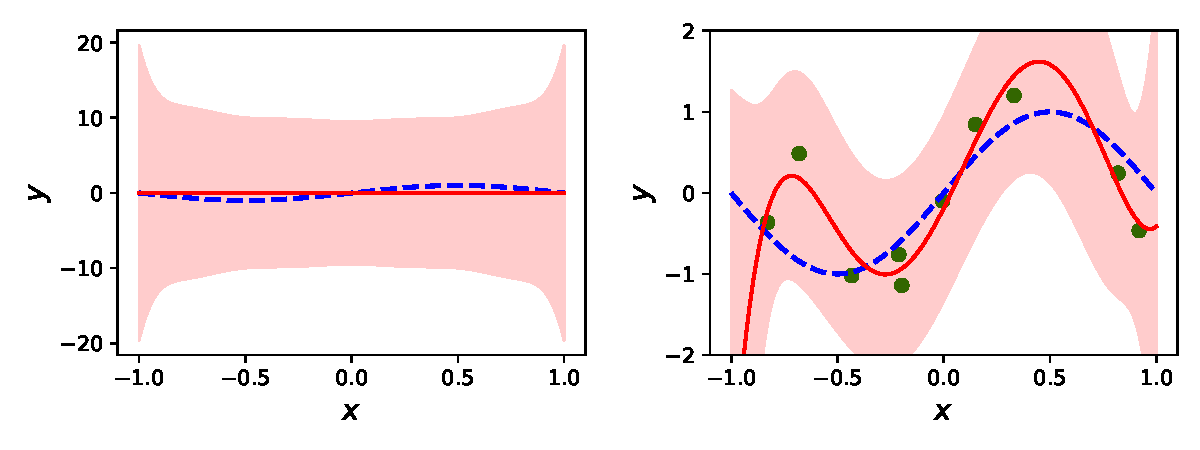
\includegraphics[width=0.9\textwidth]{../figures/bayesian_regression_1.pdf}
    \caption{10 data points}
  \end{subfigure}

  \begin{subfigure}{\textwidth}
    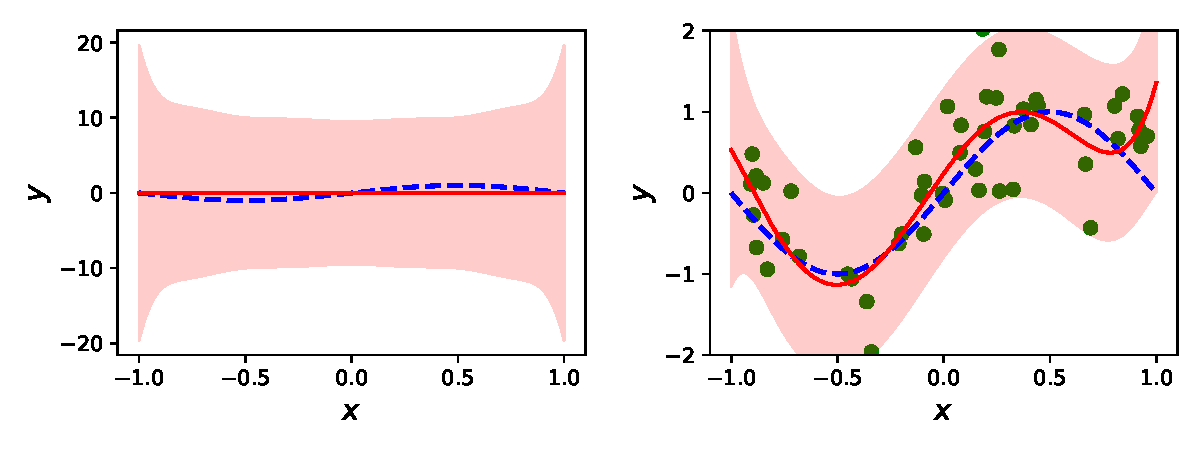
\includegraphics[width=0.9\textwidth]{../figures/bayesian_regression_2.pdf}
    \caption{50 data points}
  \end{subfigure}

  \begin{subfigure}{\textwidth}
    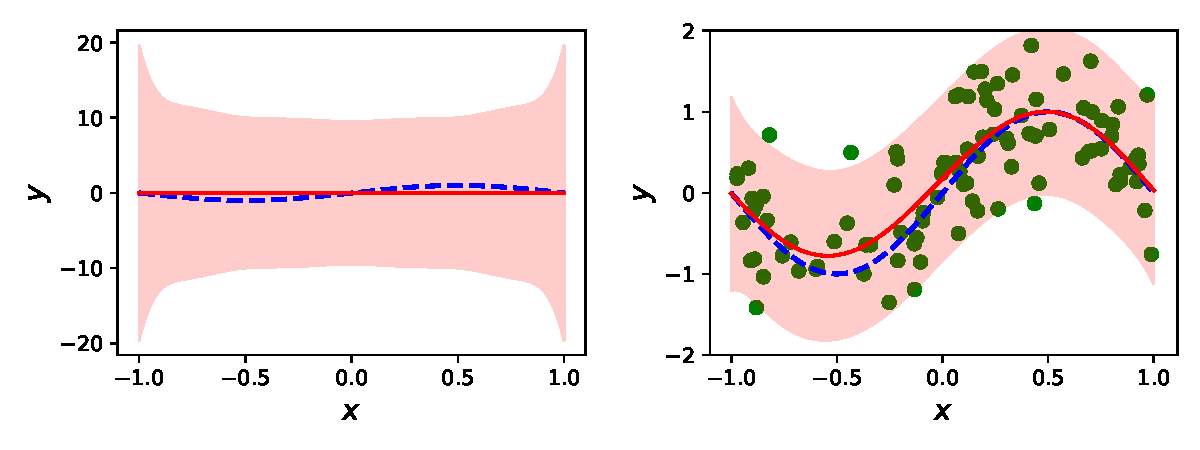
\includegraphics[width=0.9\textwidth]{../figures/bayesian_regression_3.pdf}
    \caption{100 data points}
  \end{subfigure}

  \caption{Bayesian regression with a degree 5 polynomial approximation,
  $\Vec{\theta} \sim \NormalDist(\Vec{0}, \Vec{16} \Mat{I}_6)$ prior and $\eta
  \sim \NormalDist(0, 0.25)$ noise model using different number of data points.
  The blue dashed lines represent true values, the green dots represent
  measurements, the red solid line is the mean of induced distribution on
  function values, the shaded red region is the $2\sigma$-uncertainty region of
  the same. The left panes correspond to the prior, and the right panes to the
  posterior. We observe that as the number of data points is increased, the
  posterior mean gradually approaches the true function---indicating the
  generalization error is decreasing.}
  \label{fig:regression}
\end{figure}

\subsubsection{Posterior Distribution}

From Bayes rule, we have
\begin{equation}
  \begin{split}
    -\log p(\Vec{\theta} \mid \Vec{x}, \Vec{y})
    &= -\log p(\Vec{\theta}) - \log p(\Vec{x}, \Vec{y} \mid \Vec{\theta}) +
    \text{const.} \\
    &= \frac{1}{2} (\Vec{\theta} - \Vec{\mu}_0)^\top \Mat{\Sigma}_0^{-1}
    (\Vec{\theta} - \Vec{\mu}_0) + \frac{1}{2 \sigma_\eta^2} \Norm{\Vec{y} -
    \Mat{\Phi}(\Vec{x})^\top \Vec{\theta}}^2 + \text{const.} \\
    &= \frac{1}{2} \Vec{\theta}^\top \left[\Mat{\Sigma}_0^{-1} +
    \frac{1}{\sigma_\eta^2} \Mat{\Phi}(\Vec{x}) \Mat{\Phi}(\Vec{x})^\top\right]
    \Vec{\theta} - \left[\Mat{\Sigma}_0^{-1} \Vec{\mu}_0 +
    \frac{1}{\sigma_\eta^2} \Mat{\Phi}(\Vec{x}) \Vec{y}\right]^\top \Vec{\theta}
    + \text{const.}
  \end{split}
\end{equation}
Clearly, we have
\begin{equation}
  \Vec{\theta} \mid \Vec{x}, \Vec{y} \sim \NormalDist(\Vec{\mu}, \Mat{\Sigma}),
  \quad
  \Mat{\Sigma}^{-1} = \Mat{\Sigma}_0^{-1} + \frac{1}{\sigma_\eta^2}
  \Mat{\Phi}(\Vec{x}) \Mat{\Phi}(\Vec{x})^\top,
  \quad
  \Vec{\mu} = \Mat{\Sigma} \left[\Mat{\Sigma}_0^{-1} \Vec{\mu}_0 +
  \frac{1}{\sigma_\eta^2} \Mat{\Phi}(\Vec{x}) \Vec{y}\right]
\end{equation}
and this allows us to predict the distribution of $y = \Vec{\phi}(x)^\top
\Vec{\theta} + \eta$ for any $x \in [-1, 1]$ as
\begin{equation}
  y \mid x, \Vec{x}, \Vec{y} \sim \NormalDist(\mu(x), \sigma(x)^2), \quad \mu(x)
  = \Vec{\phi}(x)^\top \Vec{\mu}, \quad \sigma(x)^2 = \Vec{\phi}(x)^\top
  \Mat{\Sigma} \Vec{\phi}(x) + \sigma_\eta^2
\end{equation}

\subsubsection{Numerical Results}

We apply this machinery to learn the function $f(x) = \sin(\pi x)$ on $[-1, 1]$.
We generate data points $(x_i, y_i)$ by first sampling $x_i$ uniformly in $[-1,
1]$, then computing $y_i = \sin(\pi x_i) + \eta_i$ with $\eta_i \sim
\NormalDist(0, 0.25)$. We assume a 5th degree polynomial expansion, and impose a
prior distribution of $\Vec{\theta} \sim \NormalDist(\Vec{0}, \sigma_\theta^2
\Mat{I}_6)$ with $\sigma_\theta = 4.0$.  In Figure~\ref{fig:regression}, we plot
the distribution of function values from the imposed prior on the parameters, as
well as the posterior after Bayesian inference.

\subsection{PAC-Bayesian Theory of Linear Regression}

While it is clear from Figure~\ref{fig:regression} that generalization error
tends to decrease as we increase the number of data points, Bayesian inference
does not provide any quantitative guarantee of this fact. This issue, however,
can be addressed in the context of PAC-Bayes learning.

We note that the likelihood term
\begin{equation}
  p(\Vec{x}, \Vec{y} \mid \Vec{\theta}) = C \exp(- \frac{1}{2 \sigma_\eta^2}
  \Norm{\Vec{y} - \Mat{\Phi}(\Vec{x})^\top \Vec{\theta}}^2)
\end{equation}
can be recovered as empirical risk $\hat{R}_S^L(\bm{\theta})$ with the loss
function
\begin{equation}
  L(\bm{\theta}, x, y) = \frac{1}{2 \sigma_\eta^2} (y - \Vec{\phi}(x)^\top
  \Vec{\theta})^2
\end{equation}
We will now show that this loss function is sub-gamma. Let us assume that the
true parameter value is $\Vec{\theta}^*$, then
\begin{equation}
  \begin{split}
    \Ev[\Vec{\theta}, x', y']{\exp(t [R_\CD^L(\Vec{\theta}) - L(\Vec{\theta},
    x', y')])}
    &= \Ev[\Vec{\theta}, x', y']{\exp(t \qty[\Ev[x, y]{L(\Vec{\theta}, x, y)} -
    L(\Vec{\theta}, x', y')])} \\
    &\leq \Ev[\Vec{\theta}]{\exp(t \Ev[x, y]{L(\Vec{\theta}, x, y)})} \\
    &= \Ev[\Vec{\theta}]{\exp(\frac{t}{2 \sigma_\eta^2} \Ev[x]{\Ev[y \mid x]{(y
    - \Vec{\phi}(x)^\top \Vec{\theta})^2}})} \\
    &= \Ev[\Vec{\theta}]{\exp(\frac{t}{2 \sigma_\eta^2}
    \qty(\Ev[x]{[\Vec{\phi}(x)^\top (\Vec{\theta} - \Vec{\theta}^*)]^2} +
    \sigma_\eta^2))} \\
    &= \Ev[\Vec{\theta}]{\exp(\frac{t}{2 \sigma_\eta^2} (\Vec{\theta} -
    \Vec{\theta}^*)^\top \Ev[x]{\Vec{\phi}(x) \Vec{\phi}(x)^\top} (\Vec{\theta}
    - \Vec{\theta}^*) + \frac{t}{2})} \\
    &\leq \Ev[\Vec{\theta}]{\exp(\frac{t}{2 \sigma_\eta^2} \kappa_{\phi, m}
    \Norm{\Vec{\theta} - \Vec{\theta}^*}^2 + \frac{t}{2})}
  \end{split}
\end{equation}
where we denote
\begin{equation}
  \kappa_{\phi, m} = \Norm{\Ev[x]{\Vec{\phi}(x) \Vec{\phi}(x)^\top}}_2
\end{equation}
We can evaluate this latest expectation with direct integration:
\begin{equation}
  \begin{split}
    \ln \Ev[\Vec{\theta}, x', y']{\exp(t [R_\CD^L(\Vec{\theta}) -
    L(\Vec{\theta}, x', y')])}
    &\leq \ln \Ev[\Vec{\theta}]{\exp(\frac{t}{2 \sigma_\eta^2} \kappa_{\phi, m}
    \Norm{\Vec{\theta} - \Vec{\theta}^*}^2 + \frac{t}{2})} \\
    &= -\frac{m}{2} \ln(1 - \frac{t \kappa_{\phi,m}
    \sigma_\theta^2}{\sigma_\eta^2}) + \frac{t \kappa_{\phi, m}}{2 \sigma_\eta^2
    - 2 t \kappa_{\phi, m} \sigma_\theta^2} \Norm{\Vec{\theta}^*}^2 +
    \frac{t}{2} \\
    &= - \frac{m}{2} \ln(1 - t c) + \frac{t c}{2 \sigma_\theta^2 (1 - t c)}
    \Norm{\Vec{\theta}^*}^2 + \frac{t}{2}
  \end{split}
\end{equation}
where $c = \kappa_{\phi, m} \sigma_\theta^2 / \sigma_\eta^2$. Now using
\begin{equation}
  - \ln(1 - x) \leq \frac{x (2 - x)}{2 (1 - x)} \quad \text{for all} \quad x \in
  [0, 1)
\end{equation}
we obtain
\begin{equation}
  \begin{split}
    \ln \Ev[\Vec{\theta}, x', y']{\exp(t [R_\CD^L(\Vec{\theta}) -
    L(\Vec{\theta}, x', y')])}
    &\leq \frac{m}{2} \frac{t c (2 - t c)}{2 (1 - t c)} + \frac{t c}{2
    \sigma_\theta^2 (1 - t c)} \Norm{\Vec{\theta}^*}^2 + \frac{t}{2} \\
    &= \frac{1}{2 (1 - t c)} \frac{m t c (2 - t c) \sigma_\theta^2 + 2 t c
    \Norm{\Vec{\theta}^*}^2 + 2 t \sigma_\theta^2 (1 - t c)}{2 \sigma_\theta^2}
    \\
    &= \frac{t^2 s^2}{2 (1 - t c)}
  \end{split}
\end{equation}
with
\begin{equation}
  s^2 = \frac{1}{t} \frac{[m c (2 - t c) + 2 (1 - t c)] \sigma_\theta^2 + 2 c
  \Norm{\Vec{\theta}^*}^2}{2 \sigma_\theta^2}
\end{equation}
Let us choose $c < 1$, then the value of $t = 1$ is acceptable, which
corresponds to $\lambda = n$. Now from Corollary~\ref{cor:alquier-sub-gamma} we
obtain
\begin{equation}
  \Ev[h \sim \rho]{R_\CD^L(h)} \leq \Ev[h \sim \rho]{\hat{R}_S^L(h)} +
  \frac{1}{n}\left[\KL{\rho}{\pi} + \ln \frac{1}{\delta}\right] +
  \frac{1}{2 (1 - c)} s^2
\end{equation}
with
\begin{equation}
  c = \frac{\kappa_{\phi, m} \sigma_\theta^2}{\sigma_\eta^2}, \quad s^2 =
  \frac{m c (2 - c) + 2 (1 - c)}{2} + \frac{c}{\sigma_\theta^2}
  \Norm{\Vec{\theta}^*}^2
\end{equation}

We now turn to estimating $\kappa_{\phi, m}$ for a specific choice of basis
functions and distribution on $x$. Let us denote
\begin{equation}
  \Mat{K} = \Ev[x]{\Vec{\phi}(x) \Vec{\phi}(x)^\top}
\end{equation}
Let us use the Legendre basis functions and uniform distribution on $[-1, 1]$;
then we have
\begin{equation}
  K_{ij} = \frac{1}{2} \int_{-1}^1 x P_{i - 1}(x) P_{j - 1}(x) \dd{x}
\end{equation}
For $i = 1$ we get $P_{i - 1}(x) = 1$, hence
\begin{equation}
  K_{1j} = \frac{1}{2} \int_{-1}^1 x P_{j - 1}(x) \dd{x} = \frac{1}{2}
  \int_{-1}^1 P_1(x) P_{j - 1}(x) \dd{x} = \frac{1}{3} \delta_{j, 2}
\end{equation}
For $i > 1$, we have
\begin{equation}
  x P_{i - 1}(x) = \frac{1}{2 i - 1} \qty[i P_i(x) + (i - 1) P_{i - 2}(x)]
\end{equation}
and therefore
\begin{equation}
  K_{ij} = \frac{i}{(2 i - 1) (2 i + 1)} \delta_{i, j - 1} + \frac{i - 1}{(2 i -
  3) (2 i - 1)} \delta_{i - 2, j - 1}
\end{equation}
It follows that $\Mat{K}$ is a symmetric tri-diagonal matrix with entries
\begin{equation}
  K_{ii} = 0, \quad K_{i + 1, i} = K_{i, i + 1} = \frac{i}{(2 i - 1) (2i + 1)}
\end{equation}
Now, for any matrix $\Mat{A}$ we have $\Norm{\Mat{A}}_2^2 \leq \Norm{\Mat{A}}_1
\Norm{\Mat{A}}_\infty$. Also for symmetric $\Mat{A}$ we have $\Norm{\Mat{A}}_1 =
\Norm{\Mat{A}}_\infty$. It follows that for our matrix $\Mat{K}$
\begin{equation}
  \kappa_{\phi, m} = \Norm{\Mat{K}}_2 \leq \Norm{\Mat{K}}_1 = \max_{1 \leq i
  \leq k} \sum_{j = 1}^m \Abs{K_{ij}} = \frac{7}{15}
\end{equation}
by direct evaluation.

With all this, we can now state the following:

\begin{proposition}[PAC-Bayes Bound for Bayesian Linear Regression]
  Let $\CD$ be a data distribution defined over $[-1, 1] \times \RR$ as follows:
  \begin{equation}
    \CD(x, y) = \UnifDist(x \mid -1, 1) \NormalDist(y \mid \Vec{\phi}(x)^\top
    \Vec{\theta}^*, \sigma_\eta^2)
  \end{equation}
  where $\Vec{\phi}(x) = (P_0(x), \ldots, P_{m - 1}(x))$ is constructed using
  Legendre polynomials. Let $\Vec{\theta} \sim \NormalDist(\Vec{0},
  \sigma_\theta^2 \Mat{I}_m)$ be a prior distribution on the parameter set
  $\RR^m$. Then given the square loss function
  \begin{equation}
    L(\Vec{\theta}, x, y) = \frac{1}{2 \sigma_\eta^2} (y - \Vec{\phi}(x)^\top
    \Vec{\theta})^2
  \end{equation}
  and real number $\delta \in (0, 1)$, the following holds with probability at
  least $1 - \delta$ over $S \sim \CD^n$ i.i.d.
  \begin{equation}
    \Ev[h \sim \hat{\rho}]{R_\CD^L(h)} \leq \Ev[h \sim
    \hat{\rho}]{\hat{R}_S^L(h)} + \frac{1}{n}\left[\KL{\hat{\rho}}{\pi} + \ln
    \frac{1}{\delta}\right] + \frac{1}{2 (1 - c)} s^2
  \end{equation}
  where $\hat{\rho}$ is the posterior obtained from Bayesian inference and
  \begin{equation}
    c = \frac{7 \sigma_\theta^2}{15 \sigma_\eta^2}, \quad s^2 = \frac{m c (2 -
    c) + 2 (1 - c)}{2} + \frac{c}{\sigma_\theta^2} \Norm{\Vec{\theta}^*}^2
  \end{equation}
\end{proposition}

Clearly, as the number of data points $n$ is increased, the difference between
generalization error and the empirical error decreases; however they don't
converge. The difference depends on four aspects: number of data points $m$,
prior standard deviation $\sigma_\theta$, noise standard deviation
$\sigma_\eta$ and the distance of the true parameter values $\Vec{\theta}^*$
from the origin. Additionally
\begin{itemize}
  \item
    To satisfy the necessary $c < 1$ constraint, we need to balance the prior
    variance and noise variance. As the noise variance is increased, we also
    need to increase the prior variance.
  \item
    As the number of data points is increased, the distance between the
    generalization and empirical errors also increase linearly.
  \item
    As the true parameter value $\Vec{\theta}^*$ moves away from the origin, the
    gap also increases quadratically with the distance. This can be
    counterbalanced by increasing the prior variance, which requires us to
    increase the noise variance.
\end{itemize}
